\section{Визуализация}
\subsection{Определение}
Визуализация (от лат. visualis, «зрительный», англ. Visualization)~— общее название приёмов представления числовой информации или физического явления в виде, удобном для зрительного наблюдения и анализа\cite{wiki:visualization_def}.

\subsection{Пример}
\includegraphics[width=\textwidth]{chapter1/minard_map_book.jpg}

Шарль Жозеф Минар (27 марта 1781, Дижон~— 24 октября 1870, Бордо). 29 ноября 1869 года — графическая визуализация вторжения Наполеона Бонапарта в Россию в 1812 году. 20 ноября 1869 года~— карта, показывающая перемещение войск Ганнибала из Иберии (Испании) в Италию во время Второй Пунической войны. 

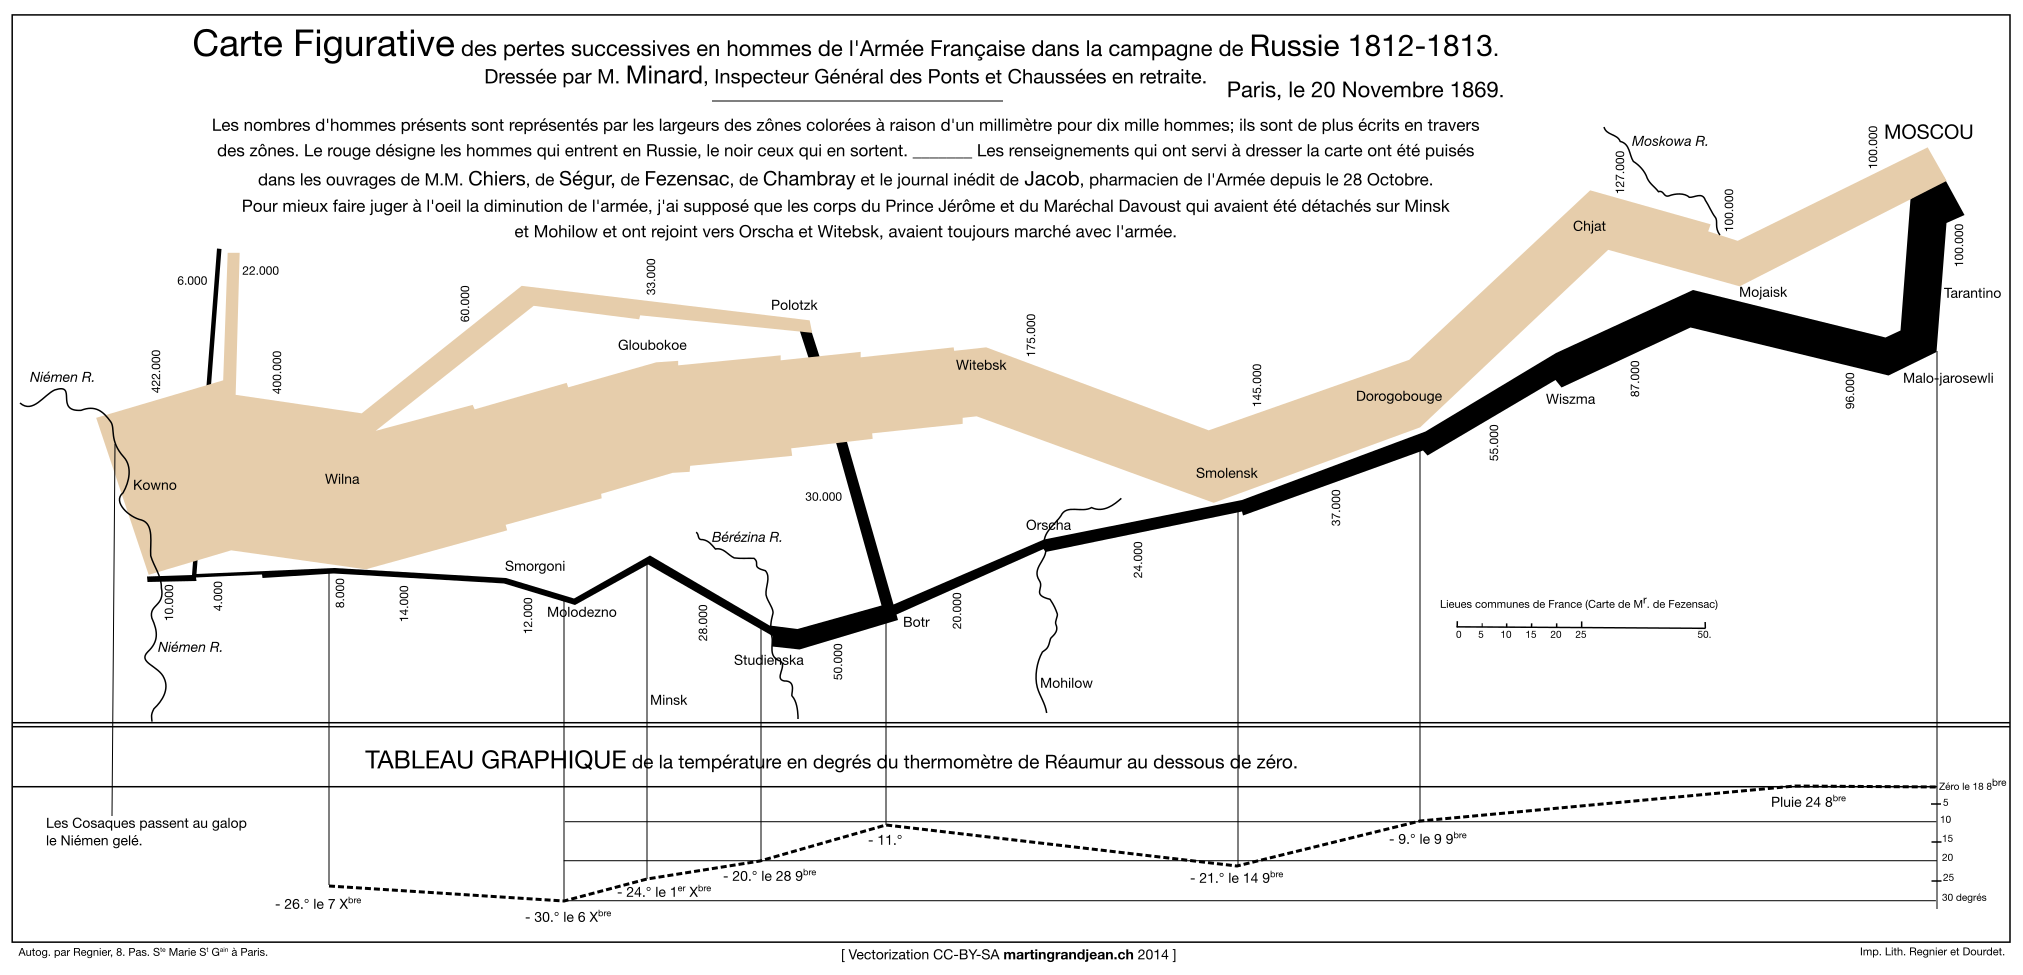
\includegraphics[width=\textwidth]{chapter1/Minard's_Map.png}

\subsection{Почему мы визуализируем?}

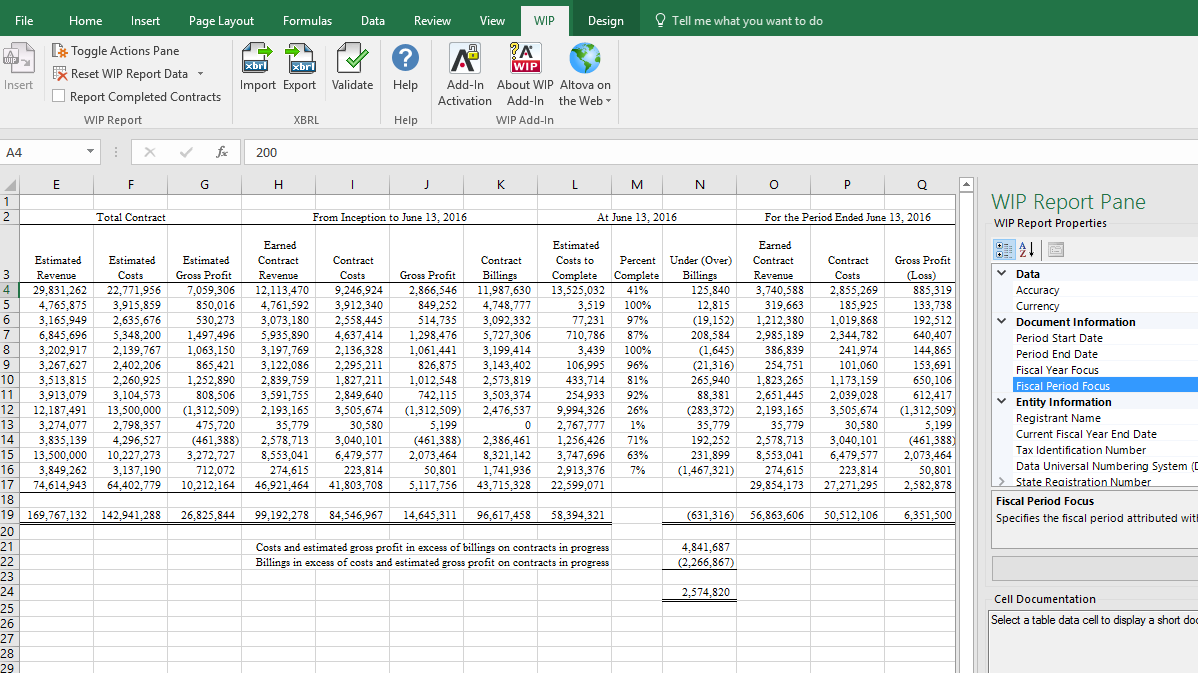
\includegraphics[width=\textwidth]{chapter1/tables-in-excel.png}

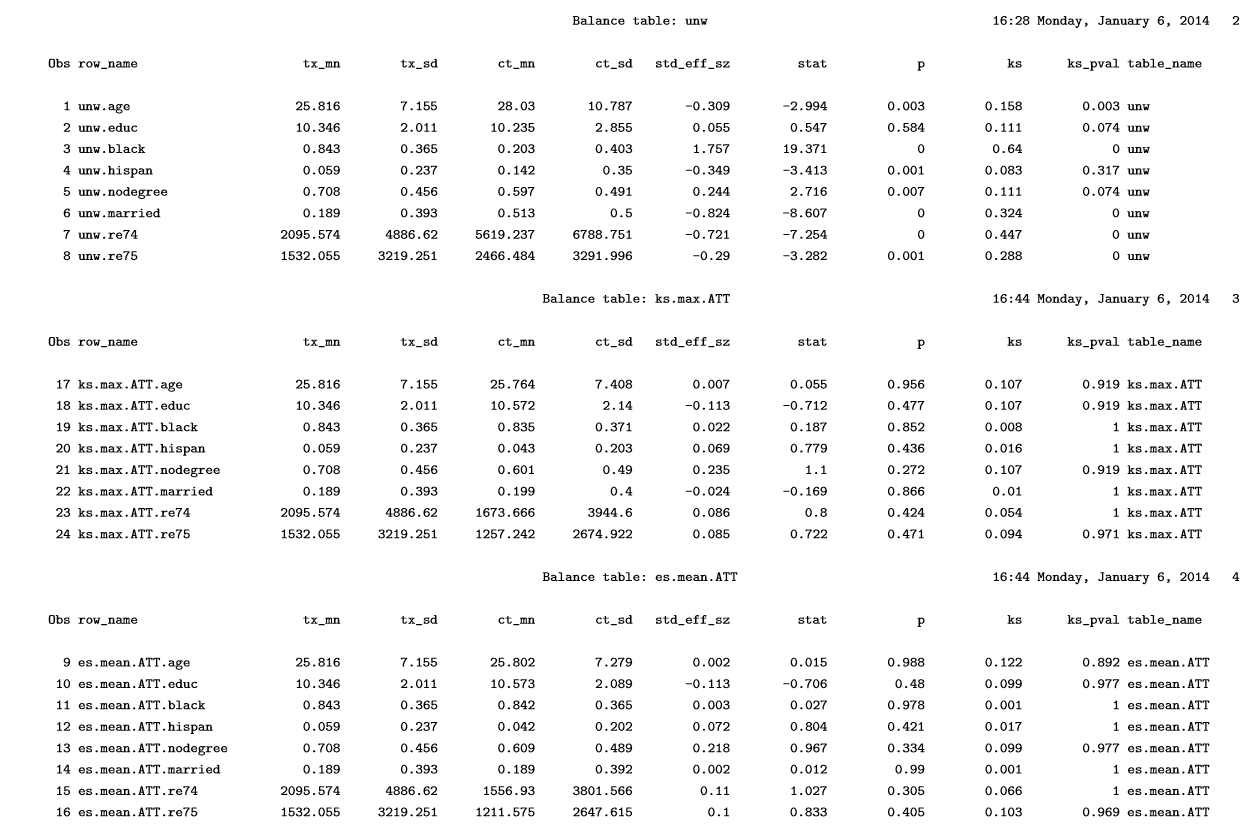
\includegraphics[width=\textwidth]{chapter1/huge-table.jpg} % SAS Macros Tutorial - https://www.rand.org/statistics/twang/sas-tutorial.html

\subsection{Попробуем сами}

\begin{wrapfigure}{r}{0.33\textwidth}
    \vspace{-0.5cm}
    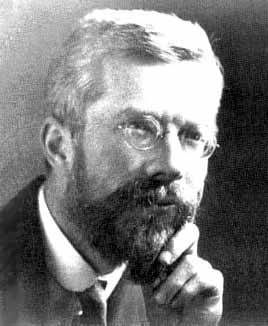
\includegraphics[width=\linewidth]{chapter1/Fischer.jpg}
     %https://upload.wikimedia.org/wikipedia/commons/4/46/R._A._Fischer.jpg
\end{wrapfigure}
Рональд Фишер в 1936 году продемонстрировал работу разработанного им метода анализа. Данные были собраны американским ботаником Эдгаром Андерсоном. \\

Признаки:
\begin{itemize}
    \item Длина наружной доли околоцветника (англ. sepal length);
    \item Ширина наружной доли околоцветника (англ. sepal width);
    \item Длина внутренней доли околоцветника (англ. petal length);
    \item Ширина внутренней доли околоцветника (англ. petal width).
\end{itemize}

\subsection{Примеры кода}

\section{Кластеризация}
\subsection{Определение}

\begin{wrapfigure}{l}{0.33\textwidth}
    \vspace{-0.5cm}
    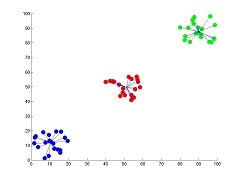
\includegraphics[width=\linewidth]{chapter1/k-means.jpg}
\end{wrapfigure}
% https://sites.google.com/site/dataclusteringalgorithms/k-means-clustering-algorithm
Кластерный анализ (англ. cluster analysis) — многомерная статистическая процедура, выполняющая сбор данных, содержащих информацию о выборке объектов, и затем упорядочивающая объекты в сравнительно однородные группы.\cite{wiki:clustering_def}

\section{Визуализация}
\subsection{Набор ирисов Фишера}

\begin{multicols}{3}
	
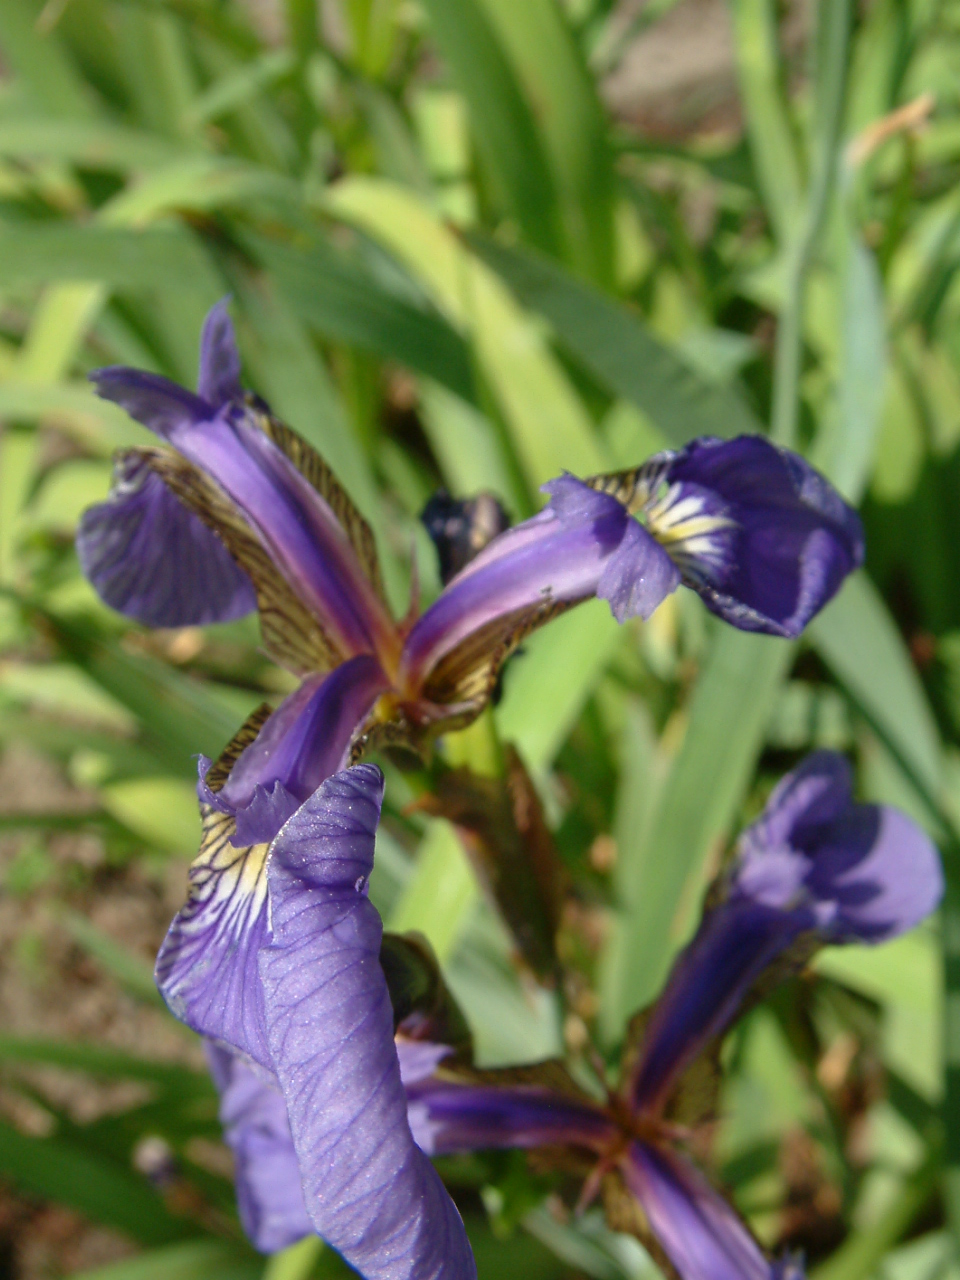
\includegraphics[height=5cm, width=4.5cm]{chapter1/Iris_setosa.jpg} %Ирис щетинистый (лат. Iris setosa)
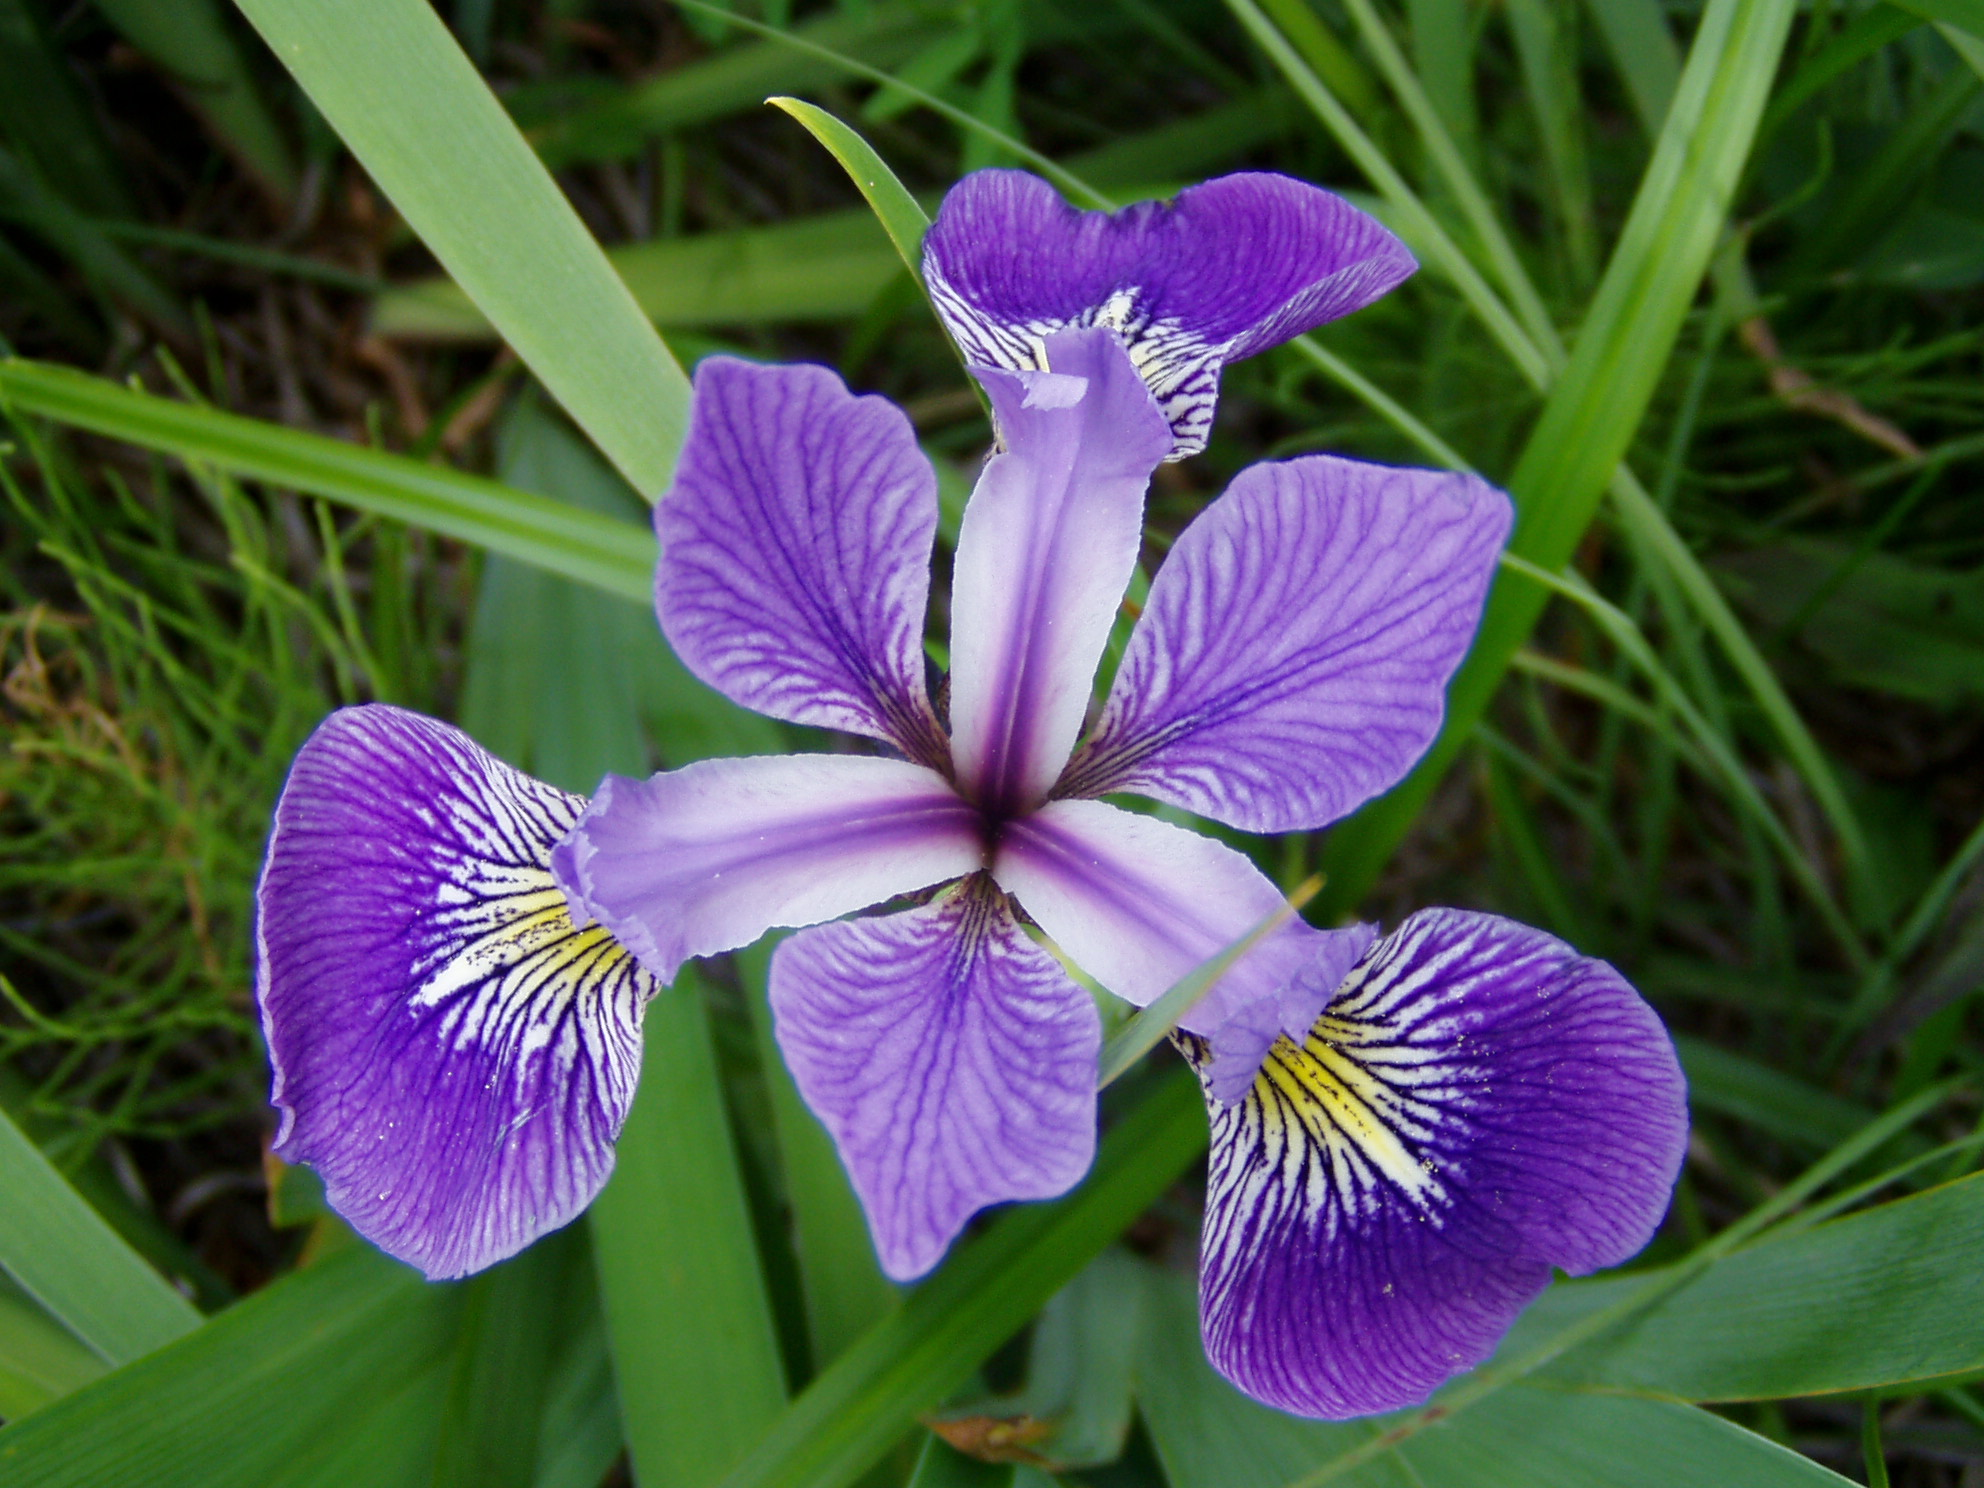
\includegraphics[height=5cm, width=4.5cm]{chapter1/Iris_versicolor.jpg} %Iris versicolor
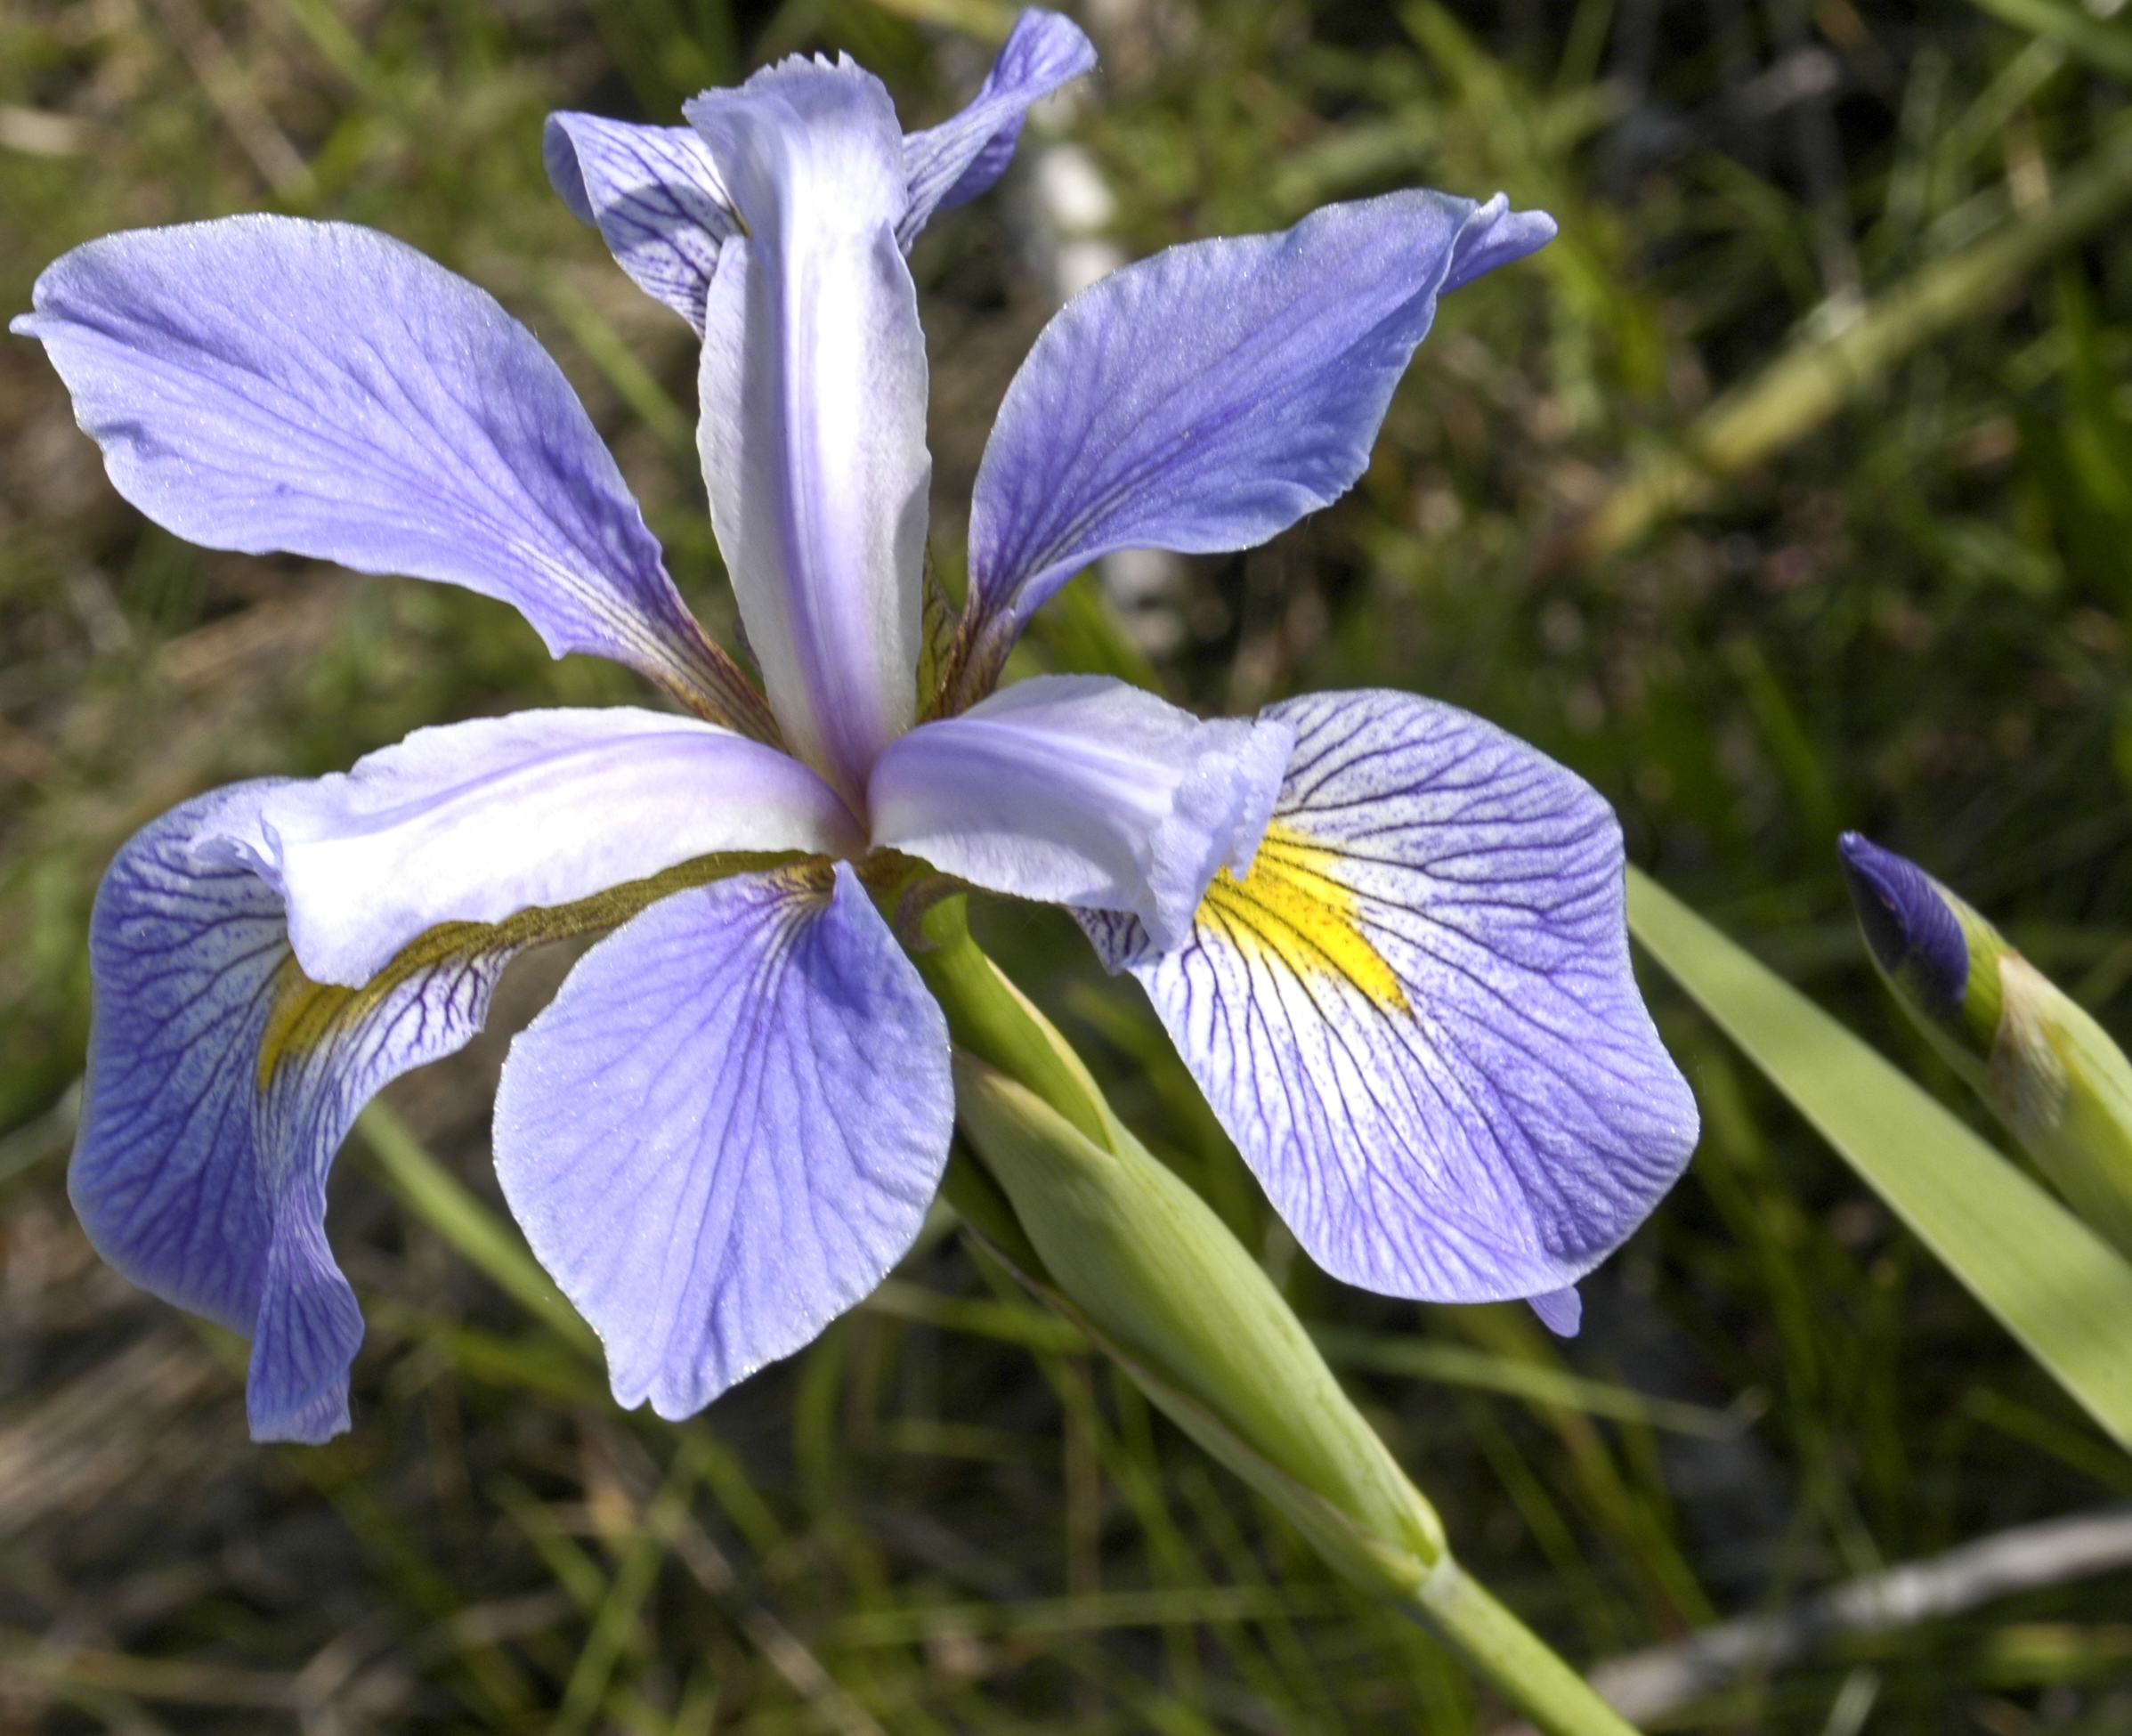
\includegraphics[height=5cm, width=4.5cm]{chapter1/Iris_virginica.jpg} %Iris virginica
\end{multicols}
    
\subsection{Примеры кода}

Задание:
\begin{itemize}
    \item Выбрать любые две пары признаков
    \item Отобразить на одном рисунке две зависимости
    \item Подписать график и оси
    \item Добавить легенду.
\end{itemize}

\section{Кластеризация}
\subsection{Методы}

Методы:
\begin{itemize}
    \item K-средних (k-means)
    \item Иерархические
\end{itemize}


\section{Машинное обучение. Определение}
Машинное обучение (англ. machine learning, ML) — класс методов искусственного интеллекта, характерной чертой которых является не прямое решение задачи, а обучение в процессе применения решений множества сходных задач. Для построения таких методов используются средства математической статистики, численных методов, методов оптимизации, теории вероятностей, теории графов, различные техники работы с данными в цифровой форме\cite{wiki:ml_def}.

Алгоритм $A$ обучается с эффективностью $E$ над данными $D$, если про росте мощности $|D|$, $E$ проявляет тенденцию к увеличению.
